%%%%%%%%%%%%%%%%%%%%%%%%%%%%%%%%%%%%%%%
% Preambulo %
%%%%%%%%%%%%%%%%%%%%%%%%%%%%%%%%%%%%%%%
\documentclass[a4paper,12pt]{article}
\usepackage[top = 2.5cm, bottom = 2.5cm, left = 2.5cm, right = 2.5cm]{geometry} 
\usepackage[T1]{fontenc}
\usepackage[utf8]{inputenc}
\usepackage{multirow}
\usepackage{booktabs} % For even nicer tables.
\usepackage{graphicx} 
\usepackage[spanish]{babel}
\usepackage{enumitem}
\usepackage{setspace}
\setlength{\parindent}{0in}
\usepackage{float}
\usepackage{fancyhdr}
\usepackage{caption} 
\DeclareCaptionLabelSeparator{none}{. }  % Quita los dos puntos
\captionsetup[figure]{labelsep=none}  % Aplica el cambio a las figuras
\captionsetup[table]{labelsep=none}   % Aplica el cambio a las tablas
\captionsetup[figure]{width=\textwidth}
\captionsetup[table]{width=\textwidth}
\usepackage{xcolor}      % Para los colores
\usepackage{fancyvrb}    % Para el entorno Verbatim 
\usepackage{enumitem} %personalizar los enumarates
\usepackage{setspace}
\usepackage{booktabs}
\usepackage{array}
\usepackage{longtable} % corta automaticamente las tablas mas grandes

% Definimos un nuevo entorno Verbatim llamado MyVerbatim
\DefineVerbatimEnvironment{MyVerbatim}{Verbatim}
	{formatcom=\color{blue}}  % Aquí puedes cambiar el color
\newcommand{\head}[1]{\textnormal{\textbf{#1}}} % comando para head
\newcommand{\normal}[1]{\multicolumn{1}{l}{#1}}
%%%%%%%%%%%%%%%%%%%%%%%%%%%%%%%%%%%%%%%%%%%%%%%%
% 3. Encabezado (y Pie de pagina)
%%%%%%%%%%%%%%%%%%%%%%%%%%%%%%%%%%%%%%%%%%%%%%%%
\pagestyle{fancy} % With this command we can customize the header style.
\fancyhf{} % This makes sure we do not have other information in our header or footer.
\lhead{\footnotesize EST526: Introducción a la Estadística No Paramétrica}
\rhead{\footnotesize Rodríguez-Flores, Zayner Edin}
%%%%%%%%%%%%%%%%%%%%%
% Pie de pagina.
%%%%%%%%%%%%%%%%%%%%%
\cfoot{\footnotesize \thepage} 
%%%%%%%%%%%%%%%%%%%%%%%%%%%%%%%%%%%%%%%%%%%%%
% Leyendas de figuras y tablas en negritas
%%%%%%%%%%%%%%%%%%%%%%%%%%%%%%%%%%%%%%%%%%%%%
\captionsetup[figure]{labelfont=bf} 
\captionsetup[table]{labelfont=bf}  
%%%%%%%%%%%%%%%%%%%%%%%%%%%%%%%%%%%%%%%%%%%%%%%%%
% Comienza documento 
%%%%%%%%%%%%%%%%%%%%%%%%%%%%%%%%%%%%%%%%%%%%%%%%%
\begin{document}
	\thispagestyle{empty} % This command disables the header on the first page. 
%%%%%%%%%%%%%%%%%%%%%%
% Encabezado
%%%%%%%%%%%%%%%%%%%%%%	
	\begin{tabular}{p{15.5cm}} % This is a simple tabular environment to align your text nicely 
	{\large \bf EST 526 Introducción a la Estadística No Paramétrica} \\
			Zayner Edin Rodríguez Flores \\ Postgrado en Edafología  \\ Colegio de Postgraduados-Campus Montecillo\\
			\hline 
			\\
	\end{tabular} % Our tabular environment ends here.
		
		\vspace*{0.1cm} % Now we want to add some vertical space in between the line and our title.
%%%%%%%%%%%%%%%%
% Titulos 		
%%%%%%%%%%%%%%%%
\begin{center} 
	{\Large \bf Tarea 2} 
			\vspace{2mm}
	
	{ \bf Prueba de \textit{Kruskal-Wallis}, Prueba de \textit{Nemenyi}, Prueba de \textit{Dunn}, ANOVA de una Vía, Prueba de \textit{Friedman}, Prueba de \textit{Ansari-Bradley}, Prueba de \textit{Kolmogorov-Smirnov}, Parcelas Divididas con \texttt{ARTools}, Coeficientes de Correlación: \textit{Pearson, Spearman, Kendall}}
			
\end{center}  
%%%%%%%%%%%%%%%
% Descripición 
%%%%%%%%%%%%%%%	
	\vspace{0.4 cm}

Para la realización de esta tarea los ejercicios se realizaron en el entorno RStudio para el lenguaje de programación R.
%%%%%%%%%%%%%%%%%%%%%%%%
% Comienzan secciones 
%%%%%%%%%%%%%%%%%%%%%%%%
%%%%%%%%%%%%%%%%%%%%%%%%%%%%%%%%%%%%%%%%%%%%%%%%%%%%%%%%%%%%%%%%%%%
\section*{Problema 1} 
La siguiente tabla contiene información sobre la longitud de las hojas de plantas de la misma especie en cada uno de cuatro lugares pantanosos no urbanizados. En cada uno de estos, se seleccionaron aleatoriamente seis plantas. \\Se seleccionaron al azar diez hojas de cada una de las plantas y la media de las diez mediciones (en centímetros) se registro para cada planta de cada uno de los lugares. Use la prueba H de Kruskal–Wallis para determinar si hay suficiente evidencia para afirmar que la distribución de las longitudes medias de las hojas difiere en localizaciones para al menos dos de los sitios. Use \(\alpha =0.05\) y encuentre el \textit{p-value} aproximado.
\\
	\begin{table}[H]
			\centering
			\caption{Longitud media de las hojas de plantas de la misma especie en cuatro lugares distintos.}
			\begin{tabular}{c|cccccc}
				\toprule[1.5 pt]
				\multicolumn{1}{c}{\head{Localización}} &
				\multicolumn{6}{c}{\head{Longitud media de la hoja (cm.)}}\\
				\midrule
				1&5.7&6.3&6.1&6.0&5.8&6.2\\
				2&6.2&5.3&5.7&6.0&5.2&5.5\\
				3&5.4&5.0&6.0&5.6&4.0&5.2\\
				4&3.7&3.2&3.9&4.0&3.5&3.6\\
				\bottomrule[1.5pt]
			\end{tabular}
			\label{tab:my_label}
	\end{table}
	\begin{enumerate} [label=\textbf{\alph*})]
\item {\textbf{Establezca el Juego de hipótesis para probar si la longitud media de las hojas son similares entre localidades.}} 
		\begin{center}
			\textcolor{blue}
				{	
				Ho=La longitud de las hojas en los cuatro sitios es igual.\\
				Ha=En al menos uno de los cuatro sitios la longitud de las hojas NO es igual.
				}
		\end{center}
\item {\textbf{Realice una gráfica de caja (Boxplot)}} 	
\begin{MyVerbatim}
# Boxplot #
ggboxplot(dat_pro1, x = "loc", y = "long",
xlab= "Localidad",ylab="Longitud media de las hojas", 
color = "loc", palette = "jco",
add = "jitter", facet.by = NULL, ggtheme = theme_pubr())
	\end{MyVerbatim}
\begin{figure}[H]
	\centering
	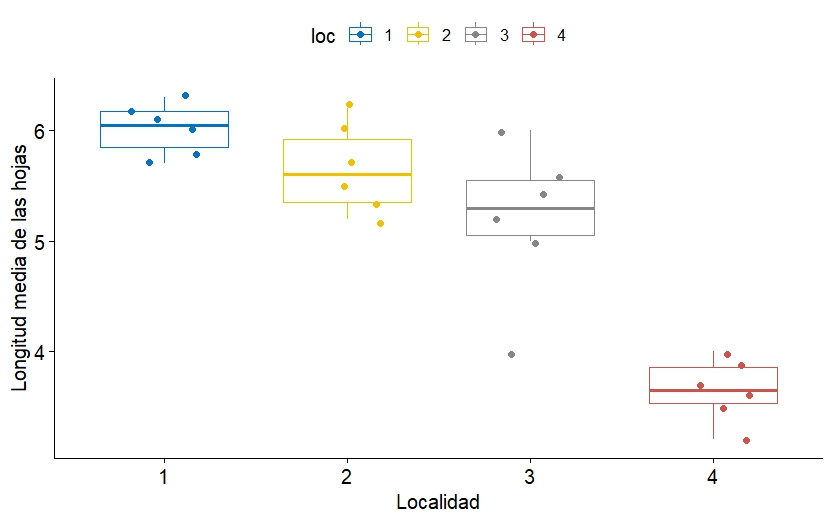
\includegraphics[width=0.7\linewidth]{Box_prob1}
	\caption[prob1_box1]{Longitud media de la hoja en cuatro diferentes localidades.}
	\label{fig:boxprob1}
\end{figure}
Resultando:\\
\item {\textbf{Utilice la prueba de Kruscal Wallis para probar la hipótesis en a) usando un \( \alpha = 0.05 \). Concluya.}}\\
	
	\begin{MyVerbatim}
# prueba de Kruscal-Wallis #
kruskal.test(long ~ loc, data = dat_pro1)
	\end{MyVerbatim}
Resultando:
\begin{MyVerbatim}
	Kruskal-Wallis rank sum test

data:  long by loc
Kruskal-Wallis chi-squared = 16.974, df = 3, p-value = 0.0007155
\end{MyVerbatim}
\textcolor{blue}{
Se concluye que hay diferencias estadísticamente significativas en la longitud de las hojas entre las localidades.}
\item {\textbf{Utilice la prueba de Nemenyi y Dunn para investigar cual es la localidad con mayor longitud usando un  \( \alpha = 0.05 \). Concluya.}}
	\begin{MyVerbatim}
library(PMCMRplus)
# Nemenyi #
kwAllPairsNemenyiTest(dat\_pro1\$long, dat\_pro1\$loc, dist = "Tukey")	
# Dunn #
kwAllPairsDunnTest(dat\_pro1\$long, dat_pro1\$loc, dist = "Tukey")
\end{MyVerbatim}
			Resultando: 
	\begin{MyVerbatim}
# Nemenyi #
Pairwise comparisons using Tukey-Kramer-Nemenyi all-pairs test with 
Tukey-Dist approximation

data: dat_pro1\$long and dat\_pro1\$loc

1      2      3     
2 0.6499 -      -     
3 0.1729 0.8164 -     
4 0.0004 0.0250 0.2117
# Dunn #
Pairwise comparisons using Dunn's all-pairs test

data: dat\_pro1\$long and dat\_pro1\$loc

1      2      3     
2 0.4876 -      -     
3 0.1635 0.4876 -     
4 0.0004 0.0239 0.1635
\end{MyVerbatim}
\textcolor{blue}{Con los datos en ambas pruebas se puede concluir que la localidad 1 es la que tiene mayor longitud de hoja y que la localidad 4 es la que menor longitud de hoja.}
\item {\textbf{Utilice el ANOVA de una vía de clasificación para probar la diferencia entre localidades usando un \( \alpha = 0.05 \).Verifique supuesto de normalidad y homocedasticidad. Concluya. Anexe una gráfica de medias}}
	\begin{MyVerbatim}
# ANOVA de una Vía 
anova1<-aov(long ~ loc, data = dat\_pro1)
summary(anova1)	
	\end{MyVerbatim}
Resultando:
	\begin{MyVerbatim}
Df Sum Sq Mean Sq F value   Pr(>F)    
loc          3 19.511   6.504   34.43 4.31e-08 ***
Residuals   20  3.778   0.189                     
Signif. codes:  0 ‘***’ 0.001 ‘**’ 0.01 ‘*’ 0.05 ‘.’ 0.1 ‘ ’ 1
	\end{MyVerbatim}
De acuerdo al p-value menor que el alpha utilizado, se concluye que existen diferencias significativas.
\begin{MyVerbatim}
# Supuestos de normalidad
	shapiro.test(anova1\$residuals)
\end{MyVerbatim}
Resultando:
	\begin{MyVerbatim}
# Shapiro-Wilk normality test
	data:  anova1\$residuals
	W = 0.95247, p-value = 0.3063
	\end{MyVerbatim}
	\begin{MyVerbatim}
# Homocedasticidad
bartlett.test(long ~ loc, data = dat\_pro1)
	\end{MyVerbatim}
Resultando:
\begin{MyVerbatim}
	Bartlett test of homogeneity of variances
	
data:  long by loc
Bartlett's K-squared = 6.3705, df = 3, p-value = 0.09491
\end{MyVerbatim}
\textcolor{blue}{Con base en los resultados anteriores, los datos cumplieron con el supuesto de normalidad en la prueba de Shapiro Wilk, asimismo con el supuesto de homocedasticidad con la prueba de Bartlet, lo que nos indica que con 5\% de nivel de significancia no existe evidencia de que las varianzas sean estadisticamente diferentes. }
	\end{enumerate}
\newpage		
%%%%%%%%%%%%%%%%%%%%%%%%%%%%%%%%%%%%%%%%%%%%%%%%%%%%%%%%%%%%%%%%%5		
\section*{Problema 2}
Stelzer et al (2012) realizaron ensayos de reacción en cadena de la polimerasa cuantitativa (qPCR) con indicadores fecales para determinar si tres laboratorios estaban proporcionando resultados similares. Se enviaron 21 muestras de fuente fecal a cada uno de los 3 laboratorios. Con las muestras como bloques. Se desea decidir si al menos un laboratorio proporcionó resultados más altos/más bajos que los demás.\\
Stelzer, E.A., Strickler, K.M., and Schill, W.B., 2012, Interlaboratory comparison of three microbial source tracking quantitative polymerase chain reaction (qPCR) assays from fecal-source and 1 environmental samples: U.S. Geological Survey Scientific Investigations Report 2012–5087, 10 p.,https://doi.org/10.3133/sir20125087.
\begin{center}
		\begin{longtable}{c|c|c}
			\caption{Contenido de bacterias totales por muestras en tres distintos laboratorios.} \label{tab:example} \\
			\hline
			\textbf{Bacterias Totales} & \textbf{Muestra} &\textbf{Laboratorio }\\
			\hline
			\endfirsthead
			\hline
			Bacterias Totales & Muestra & Laboratorio \\
			\hline
			\endhead
			\hline
			\endfoot
			\hline
			\endlastfoot
			44  & 1  & 1  \\
			42  & 2  & 1  \\
			180 & 3  & 1  \\
			200 & 4  & 1  \\
			190 & 5  & 1  \\
			200 & 6  & 1  \\
			190 & 7  & 1  \\
			48  & 8  & 1  \\
			54  & 9  & 1  \\
			33  & 10 & 1  \\
			57  & 11 & 1  \\
			55  & 12 & 1  \\
			44  & 13 & 1  \\
			53  & 14 & 1  \\
			60  & 15 & 1  \\
			127 & 16 & 1  \\
			3000& 17 & 1  \\
			620 & 18 & 1  \\
			1300& 19 & 1  \\
			170 & 20 & 1  \\
			170 & 21 & 1  \\
			45  & 1  & 2  \\
			40  & 2  & 2  \\
			190 & 3  & 2  \\
			210 & 4  & 2  \\
			180 & 5  & 2  \\
			190 & 6  & 2  \\
			190 & 7  & 2  \\
			49  & 8  & 2  \\
			54  & 9  & 2  \\
			32  & 10 & 2  \\
			56  & 11 & 2  \\
			53  & 12 & 2  \\
			43  & 13 & 2  \\
			51  & 14 & 2  \\
			59  & 15 & 2  \\
			120 & 16 & 2  \\
			3000& 17 & 2  \\
			620 & 18 & 2  \\
			1200& 19 & 2  \\
			170 & 20 & 2  \\
			170 & 21 & 2  \\
			120 & 1  & 3  \\
			99  & 2  & 3  \\
			480 & 3  & 3  \\
			480 & 4  & 3  \\
			470 & 5  & 3  \\
			390 & 6  & 3  \\
			410 & 7  & 3  \\
			120 & 8  & 3  \\
			130 & 9  & 3  \\
			70  & 10 & 3  \\
			140 & 11 & 3  \\
			130 & 12 & 3  \\
			98  & 13 & 3  \\
			120 & 14 & 3  \\
			140 & 15 & 3  \\
			320 & 16 & 3  \\
			7200& 17 & 3  \\
			1500& 18 & 3  \\
			2900& 19 & 3  \\
			450 & 20 & 3  \\
			360 & 21 & 3  \\
			\end{longtable}
		\end{center}
\begin{enumerate} [label=\textbf{\alph*})]
\item {\textbf{Indique la hipótesis nula y alterna para la prueba de \textit{Friedman} en este problema.}}
	\begin{center}
		\textcolor{blue}{
			Ho: Los resultados entre los laboratorios son iguales entre sí.\\
			Ha: Los resultados entre los laboratorios son diferentes entre sí.}
	\end{center}
\item {\textbf{Obtenga el estadístico de \textit{Friedman} y pruebe Ho usando \(\alpha=0.05\).}}
	\begin{MyVerbatim}
# Friedman Test #
friedman.test(prob2\$bac\_tot, prob2\$num,\_lab, prob2\$muestra)
	\end{MyVerbatim}
Resultando:
\begin{MyVerbatim}
# Friedman rank sum test
	
data:  prob2\$bac\_tot, prob2\$num\_lab and prob2\$muestra
Friedman chi-squared = 3.1795, df = 2, p-value = 0.204
\end{MyVerbatim}
\textcolor{blue}{De acuerdo a la prueba anterior, se rechaza la Ho de que los resultados de los laboratorios son iguales entre si y se concluye que al menos los resultados de un laboratorio es diferente a los demás.}
\item {\textbf{Use una prueba de comparación múltiple para determinar que laboratorios difieren de otros. Apoye su decisión usando gráficos}}\\
\textcolor{blue}{Se realizó una interpretación gráfica boxplot y designando letras para la comparación de medias producto de la prueba post hoc de Nemenyi, que nos permite distinguir la diferencia entre los grupos (laboratorios).}
	\begin{MyVerbatim}
	# Test post hoc Nemenyi #
nemenyi\_result <- frdAllPairsNemenyiTest(bac\_tot ~ num\_lab | muestra, 
data = prob2)
print(nemenyi\_result)

	# Extraer las letras de comparación de medias #
nemenyi\_letters <- multcompLetters(nemenyi\_result\$p.value)
print(nemenyi\_letters)

	# Data frame con las letras para ggplot #
nemenyi\_summary <- data.frame(num\_lab = names(nemenyi\_letters\$Letters), 
Letters = nemenyi\_letters\$Letters)

	# Boxplot con letras de comparación de medias #
ggplot(prob2, aes(x = num\_lab, y = bac\_tot, fill = num\_lab)) +
geom\_boxplot() +
geom\_text(data = nemenyi\_summary, 
aes(x = num\_lab, y = max(prob2\$bac\_tot) + 1, label = Letters),
vjust = 0) +
labs(title = "Comparación de Medias de tres Laboratorios",
x = "Número de Laboratorio",
y = "Bacterias Totales") +
theme\_pubr()
	\end{MyVerbatim}
Resultando:
\begin{figure}[H]
	\centering
	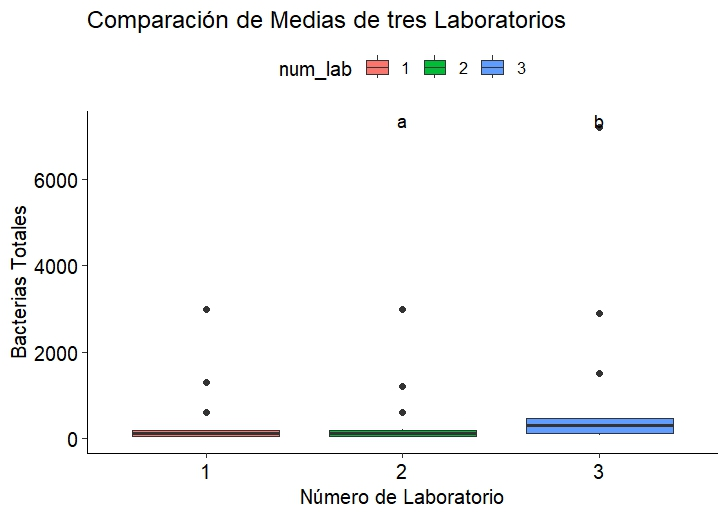
\includegraphics[width=0.7\linewidth]{Med_prob2}
	\caption[boxmedias]{Comparación de medias entre laboratorios.}
	\label{fig:medprob2}
\end{figure}
\textcolor{blue}{De acuerdo con el gráfico anterior se puede observar que si existe una diferencia estadística significativa y el laboratorio 3 es el que tiene una media superior a los otros dos laboratorios. Afirmando el resultado en la prueba de \textit{Friedman}.}
\end{enumerate}
	
\newpage
%%%%%%%%%%%%%%%%%%%%%%%%%%%%%%%%%%%%%%%%%%%%%%%%%%%%%%%%%%%%%%%%%%%%%%%%%%%%%%
\section *{Problema 3}
Se diseñó una serie de experimentos para comprobar la hipótesis de que la siembra masiva de yoduro de plata puede, en determinadas condiciones, provocar un aumento de las precipitaciones. \\
Los datos de estos experimentos se publicaron en el artículo "\textit{A Bayesian Analysis of a Multiplicative Treatment Effect in Weather Modification" [Technometrics (1975) 17:161-166]}. Aquí se informa del volumen de lluvia que cae de la nube tras la siembra con yoduro de plata.
	\begin{table}[H]
		\centering
		\caption{Tabla de datos de siembra de nubes.}
		\begin{tabular}{cccccccc}
			\toprule[1.5 pt]
			\multicolumn{8}{c}{\head{Rainfall (acre-feet)Unseeded Clouds (RCU)}} \\
			\midrule
			129.6&31.4&2745.6&489.1&430&302.8&119&4.1\\
			92.4&17.5&200.7&274.7&274.7&7.7&1656&978\\
			198.6&703.4&1697.8&334.1&118.3&255&115.3&242.5\\
			32.7&40.6&&&&&&\\
			\midrule
			\multicolumn{8}{c}{\head{Rainfall (acre-feet)Seeded Clouds (RSC)}} \\
			\midrule
			26.1&26.3&87&95&372.4&0&17.3&24.4\\
			11.5&321.2&68.5&81.2&47.3&28.6&830.1&345.5\\
			1202.6&36.6&4.9&4.9&41.1&29&163&244.3\\
			147.8&21.7&&&&&&\\
			\bottomrule[1.5pt]
		\end{tabular}
		\label{tab:my_label3}
\end{table}
\begin{enumerate} [label=\textbf{\alph*})]
	\item Use la prueba de Ansari-Bradley para probar si la variabilidad en ambos tratamientos es igual, establezca
	su juego de hipótesis, gráficos y conclusiones con \(\alpha =0.05\).
\begin{center}
	\textcolor{blue}{Ho: La variabilidad de lluvias en ambos casos es igual.\\
	Ha: La variabilidad de lluvias en ambos casos no es igual.}
\end{center}
\textcolor{blue}{Como primer impresión se realiza una grafica boxplot (Figura 3). Código siguiente:}
\begin{MyVerbatim}
# Gráfica boxplot #
ggboxplot(dat3, x = "trat", y = "rain",
 xlab= "Tratamiento",ylab="Lluvia (mm)", 
 color = "trat", palette = "jco",
 add = "jitter", facet.by = NULL, 
 ggtheme = theme_pubr())
\end{MyVerbatim}
\begin{figure}[H]
	\centering
	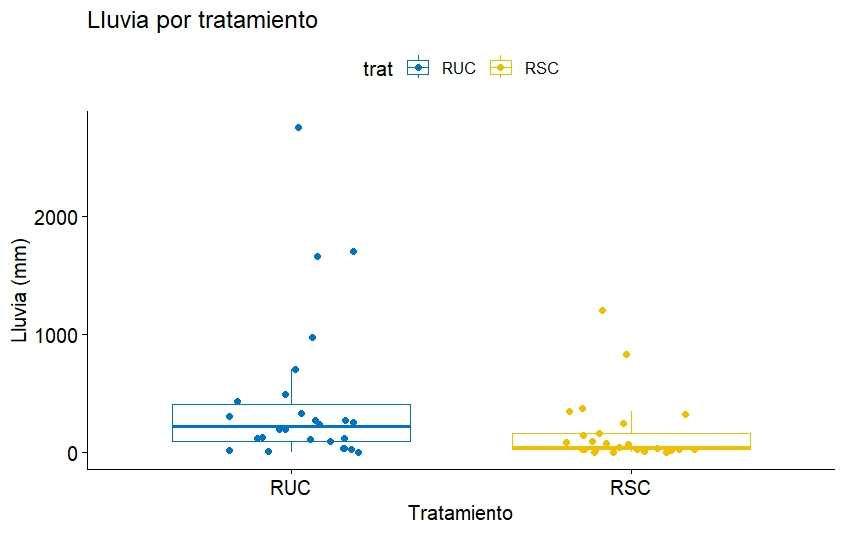
\includegraphics[width=0.7\linewidth]{lluv_box3}
	\caption[lluv_box]{Precipitación (mm) por tratamiento.RUC:Rainfall Unseeded Clouds; RSC:Rainfall Seeded Clouds}
	\label{fig:lluvbox3}
\end{figure}
En la gráfica anterior se puede observar que existe una diferencia mínima visualmente en la distribución y media de los datos de cada uno de los tratamientos. Sin embargo, para poder concluir con certeza una diferencia estadistica entre ambos casos se realiza a continuación la prueba de \textit{Ansari-Bradley} y \textit{Kolmogorv-Smirnov}.
\begin{MyVerbatim}
# Prueba de Ansari-Bradley
ansari.test(rain~trat,dat3, var.equal=TRUE,alternative="two.sided", 
alpha=0.05)
\end{MyVerbatim}
Resultando:
\begin{MyVerbatim}
	Ansari-Bradley test
data:  rain by trat
AB = 344, p-value = 0.7976
alternative hypothesis: true ratio of scales is not equal to 1
\end{MyVerbatim}
De acuerdo a la prueba anterior y con un \(\alpha=0.05\), se puede concluir que no existe diferencia estadísticamente significativas  en la varianza de las lluvias entre ambos tratamientos.
\item Use la prueba de Kolmogorov-Smirnov para probar si las distribuciones de precipitación son iguales en ambos tratamientos, use \(\alpha=0.05\).

\begin{MyVerbatim}
# Prueba de  Kolmogorov-Smirnov
ks.test(rain~trat,dat3,alternative="two.sided")	
\end{MyVerbatim}
Resultando:
\begin{MyVerbatim}
Exact two-sample Kolmogorov-Smirnov test

data:  rain by trat
D = 0.42308, p-value = 0.01774
alternative hypothesis: two-sided
\end{MyVerbatim}
De la misma manera que con la pruena de \textit{Ansari-Bradley}, con un \(\alpha=0.05\), se puede concluir que no existe diferencia estadísticamente significativas en distribución de la de las lluvias entre ambos tratamientos.
\end{enumerate}

\newpage
%%%%%%%%%%%%%%%5
\section*{Problema 4}
Nappi (E12) investigó los cambios que se producen en los hemocitos de larvas de \textit{Drosophila algonquin} durante la parasitación por el himenóptero parásito (parasitoide) \textit{Pseudocoila bochei}. Diez y siete horas después de la parasitación de larvas de \textit{Drosophila algonquin}, se efectuaron recuentos diferenciales (\%) de plasmocitos en tres grupos: larvas hospedadoras en las que la reacción fue satisfactoria (S), larvas en las que la reacción no fue satisfactoria (U) y larvas en las que no hubo reacción visible del hospedador (N). Los resultados se muestran en la Tabla 6.16. Se desea comprobar la hipótesis nula de que no hay diferencia entre los tres grupos frente a la alternativa de que los recuentos diferenciales de plasmatocitos (\%) disminuyen en los tres grupos del grupo N al grupo S.
\begin{center}
	\begin{table}[H]
		\centering
		\caption{Differential plasmocyte counts, percent from larvae of \textit{Drosophila algonquin} 27 hours after parasitization by \textit{Pseudecoila bochei} (host age 91 hours ehen parasitized).}
		\begin{tabular}{ccc}
			\toprule[1.5 pt]
			Successful host reactions (S) & Unsuccessful host reactions (U)& No visible host reactions (N) \\
			\midrule
			54.0&79.8&98.6\\
			67.0&82.0&99.5\\
			47.2&88.8&95.8\\
			71.1&79.6&93.3\\
			62.7&85.7&98.9\\
			44.8&81.7&91.1\\
			67.4&88.5&94.5\\
			80.2&&\\
			\bottomrule[1.5pt]
		\end{tabular}
		\label{tab:my_label4}
	\end{table}
\end{center}
\begin{enumerate}  [label=\textbf{\alph*})]
\item \textbf{Use la prueba de Jonckheere-Terpstra, escriba el juego de hipótesis y concluya \(\alpha=0.05\).}\\
\begin{center}
\textcolor{blue}{Ho: No hay diferencias entre los tres grupos.\\
Ha: Los recuentos diferenciales de plasmocitos (\%) disminuyen en los tres grupos, del grupo N al grupo S.}
\end{center}
Prueba de Jonckheere-Terpstra:
\begin{MyVerbatim}
# Prueba de Jonckheere-Terpstra #
jonckheereTest(prob4\$counts, prob4\$groups, alternative = "greater")	
\end{MyVerbatim} 
Resultado:
\begin{MyVerbatim}
Jonckheere-Terpstra test

data:  prob4\$counts and prob4\$groups
z = 4.7259, p-value = 1.146e-06
alternative hypothesis: greater
sample estimates:
JT 
159
\end{MyVerbatim}
\textcolor{blue}{De acuerdo a la prueba anterior se rechaza la hipótesis nula, por lo que se puede decir que existe una diferencia entre los grupos ya que el valor de p-value, es menor al \(\alpha=0.05\).}\\
\textcolor{blue}{Ademas de observar que una tendencia creciente en la variable counts del grupo S al N (Figura 4).}
\begin{figure}[H]
	\centering
	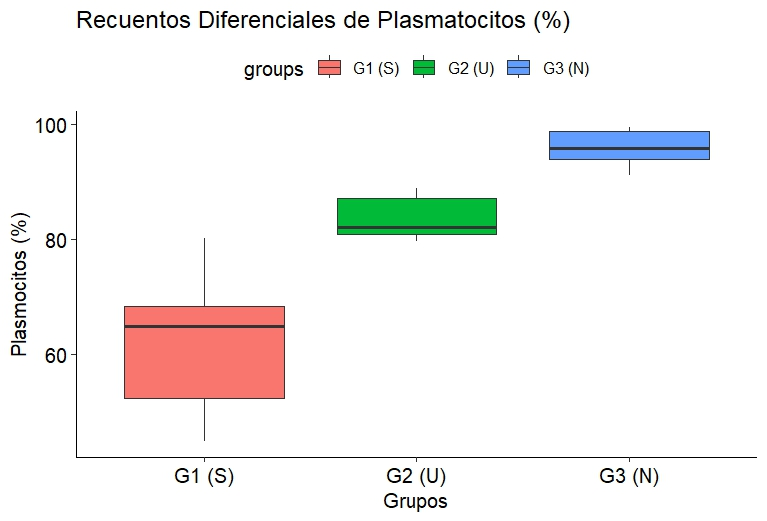
\includegraphics[width=0.7\linewidth]{RDP_prob4}
	\caption[RDPprob4]{Porcentaje de recuentos de plasmatocitos para los tres grupos.}
	\label{fig:rdpprob4}
\end{figure}
\end{enumerate}
\newpage
%%%%%%%%%%%%%%%%%%%%%%%%%%%%%%%%%%%%%%%%%%%%%%%%%%%%%%%%%%%%%
\section*{Problema 5}
Del articulo: \\
\\Edward Durner,2019. Effective Analysis of Interactive Effects with Non Normal Data Using the Aligned Rank Transform, ARTool and SAS University Edition, \textit{Horticulturae 2019}, 5, 57; doi:10.3390/horticulturae5030057.\\
\\Escribir un reporte: con tablas gráficos interpretación y conclusiones.\\
\\Consideraciones: consider an experiment where six rates of three nitrogen sources were evaluated for strawberry yield (g·plant-1). The experimental design was a split plot with nitrogen source as the main plot and nitrogen rate as the sub-plot. There were five replicates of the main plot and the main plots were set in a randomized complete block design.\\
\begin{enumerate}[label=\textbf{\alph*})]
\item Analice los datos para un modelo de parcelas divididas en forma paramétrica.
\item Utilizando el modelo de parcelas divididas (paramétrico).
	\begin{MyVerbatim}
# Parcelas divididas (paramétrico) #
# Análisis de varianza #
anova_par_div<-aov(Yield ~ blk+ Nitrogen*Rate + 
Error(blk:Nitrogen), data = datos3)
summary(anova_par_div)
	\end{MyVerbatim}
Resultando:
	\begin{MyVerbatim}
Error: blk:Nitrogen
         Df Sum Sq Mean Sq
blk       1  891.1   891.1
Nitrogen  2   67.8    33.9
Error: Within
	      Df Sum Sq Mean Sq F value Pr(>F)
Nitrogen       2   2533  1266.7   1.587    0.214
Rate           1      3     3.2   0.004    0.950
Nitrogen:Rate  2    785   392.6   0.492    0.614
Residuals     51  40696   798.0
	\end{MyVerbatim}
\textcolor{blue}{De acuerdo a la prueba anterior, se puede concluir que no existio algun efecto de los tratamientos y su combinación, dado que todos los pvalue se encontraron por encima del alfa (\(\alpha=0.05\)).}

\item Pruebe los efectos de tratamientos y la interacción tratamiento vs tiempo, use \(\alpha=0.5\). Verifique supuestos.

\begin{center}
	Comprobación de supuestos
\end{center}
\textit{Independencia}\\
De una manera visual, podemos comprobar la normalidad de los datos mediante gráficos qqline. 
Estos gráficos muestra que en las 3 Variedades se pudiera suponer normalidad; sin embargo,
es necesario establecer el juego de hipótesis. 
\begin{MyVerbatim}
par(mfrow = c(2,2))
qqnorm(datos3[datos3$Rate=="1","Yield" ], main="Var1")
qqline(datos3[datos3$Rate=="1","Yield" ])
qqnorm(datos3[datos3$Rate=="2","Yield" ], main="Var2")
qqline(datos3[datos3$Rate=="2","Yield" ])
qqnorm(datos3[datos3$Rate=="3","Yield" ], main="Var3")
qqline(datos3[datos3$Rate=="3","Yield" ])
qqnorm(datos3[datos3$Rate=="4","Yield" ], main="Var4")
qqline(datos3[datos3$Rate=="4","Yield" ])
par(mfrow = c(1,1))
\end{MyVerbatim}
\begin{figure}[H]
	\centering
	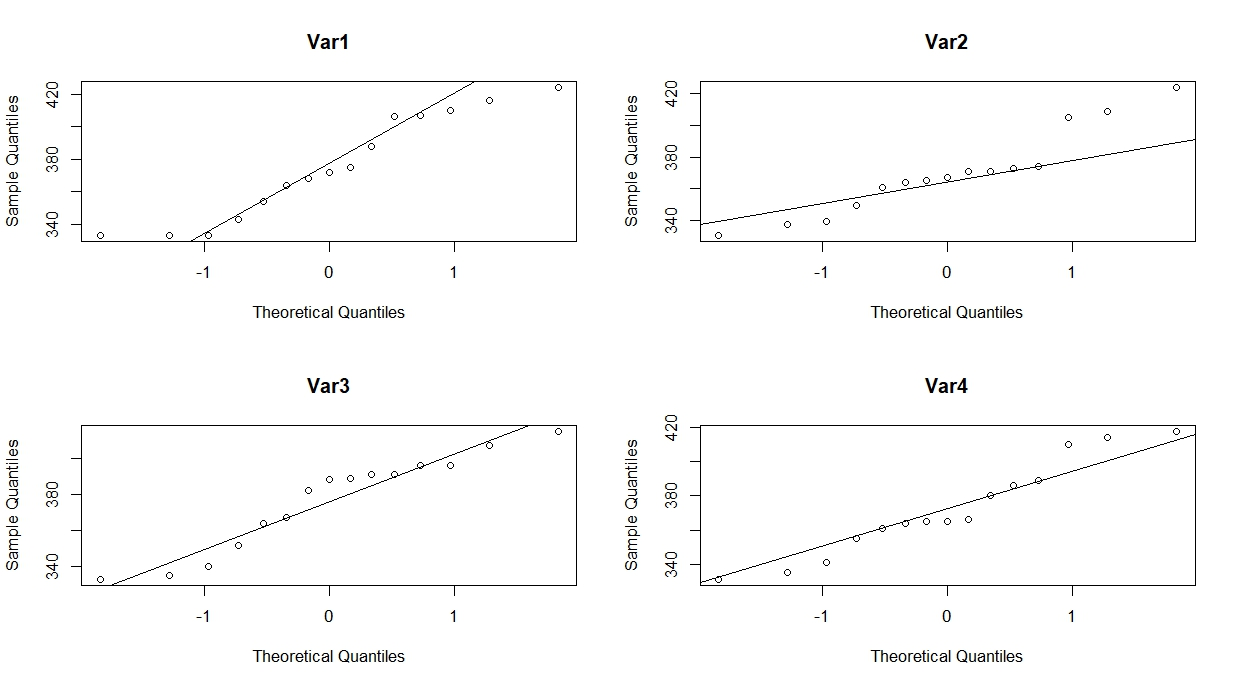
\includegraphics[width=0.7\linewidth]{prob5_qqline}
	\caption[prob5_qqline]{Gráficos qqline, para verificación de independencia de los datos.}
	\label{fig:prob5qqline}
\end{figure}
\textit{Test de hipótesis} \\
\\\textcolor{blue}{Dado que los grupos tienen mas de 50 observaciones se emplea el test de Kolmogorov-Smirnov con la corrección de Lilliefors.}
\begin{MyVerbatim}
by(data = datos3,INDICES = datos3$Rate,
FUN = function(x){ lillie.test(x$Yield)})
\end{MyVerbatim}

\begin{MyVerbatim}
datos3$Rate: 1

Lilliefors (Kolmogorov-Smirnov) normality test

data:  x$Yield
D = 0.16597, p-value = 0.3232

------------------------------------------------ 
datos3$Rate: 2

Lilliefors (Kolmogorov-Smirnov) normality test

data:  x$Yield
D = 0.22944, p-value = 0.03258

------------------------------------------------ 
datos3$Rate: 3

Lilliefors (Kolmogorov-Smirnov) normality test

data:  x$Yield
D = 0.20357, p-value = 0.095

------------------------------------------------ 
datos3$Rate: 4

Lilliefors (Kolmogorov-Smirnov) normality test

data:  x$Yield
D = 0.18674, p-value = 0.1711
	\end{MyVerbatim}

\textcolor{blue}{De esta manera se puede observar que todas las variedes cumplen con el supuesto. Sin ebargo para Rate 2, esta casi en el limite para aceptar que se distribuye de forma normal.}\\

\textit{Homocedasticidad}\\
	
\textcolor{blue}{Tomando en cuenta que hay un grupo (Rate 2) que se encuentra en el límite para aceptar que se distribuye de forma normal el test de Fisher y el de Bartlett no son recomendables. En su lugar es mejor emplea un test basado en la mediana test de Levene o test de Fligner-Killeen.}

\begin{MyVerbatim}
fligner.test(Yield ~ Rate, data = datos3)
\end{MyVerbatim}
Resultando:
\begin{MyVerbatim}
Fligner-Killeen test of homogeneity of variances
	
data:  Yield by Rate
Fligner-Killeen:med chi-squared = 0.86664, df = 3, p-value = 0.8335
\end{MyVerbatim}

\textcolor{blue}{Con una confiabilidad de 95 \% y de acuerdo con el test de Fligner-Killeen con un p-value de 0.8335 se acepta la hipótesis de homocedasticidad;es decir, las varianzas son iguales.}

\item Utilice el método de Tukey para investigar cual es el mejor tratamiento.
\begin{MyVerbatim}
# Prueba de Tukey #
anova_simplified <- aov(Yield ~ blk + Nitrogen * Rate, data = datos3)

tukey_result <- TukeyHSD(anova_simplified)
tukey_result
plot(tukey_result)
\end{MyVerbatim}
\begin{figure}[H]
	\centering
	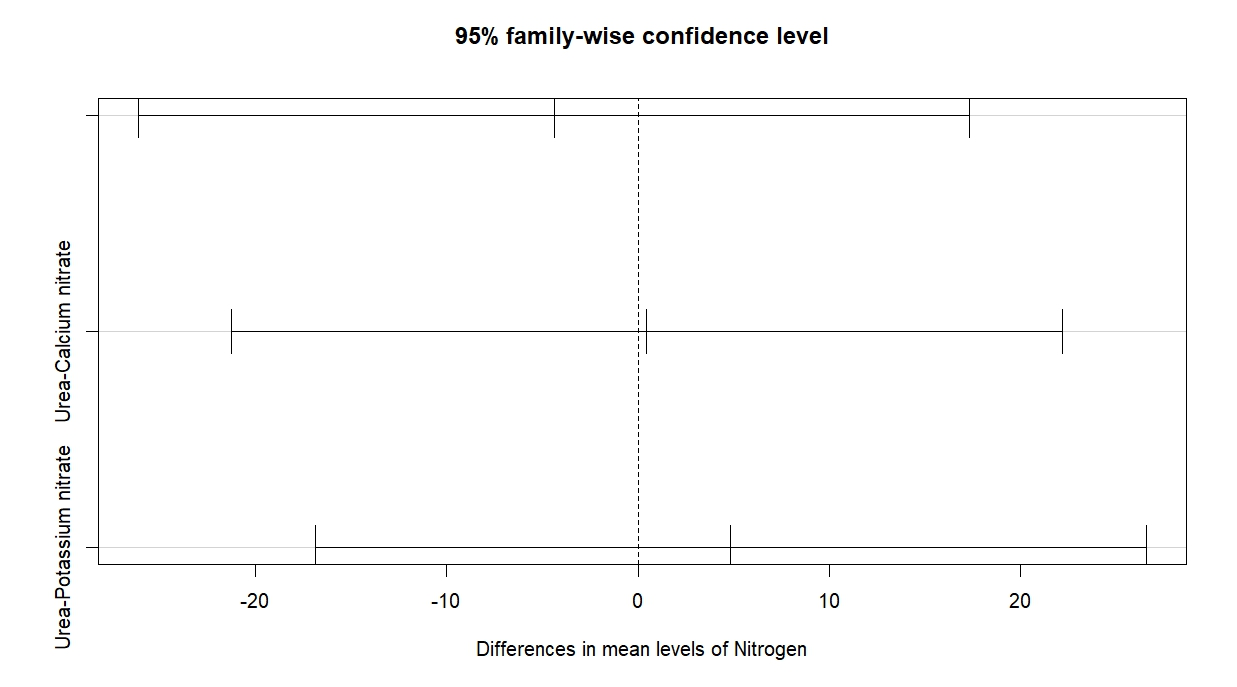
\includegraphics[width=0.7\linewidth]{prob5_tuke}
	\caption[prob5_tukey]{Grafíco de la comparación de medias Tukey \(\alpha=0.05)\).}
	\label{fig:prob5tuke}
\end{figure}
\textcolor{blue}{En la Figura anterior, se puede observar que el efecto de los niveles de nitrógeno tienen medias muy parecidas entre si, dado que se encuentran cerca de la media.}
\item Realizar la gráfica de interacción nit*rate e interpretar.
\begin{MyVerbatim}
# Grafico de interacción #
interaction.plot(datos3$Nitrogen, datos3$Rate, datos3$Yiel)
interaction.plot(datos3$Nitrogen, datos3$Rate, datos3$Yield,
type = "l",    
ylab= "Yield",
xlab = "Nitrogen",
col = c("blue4", "red4","green","orange"),
lty = 1,  
lwd = 2, 
trace.label = "Rate",
xpd = FALSE)
\end{MyVerbatim}
\begin{figure}[H]
	\centering
	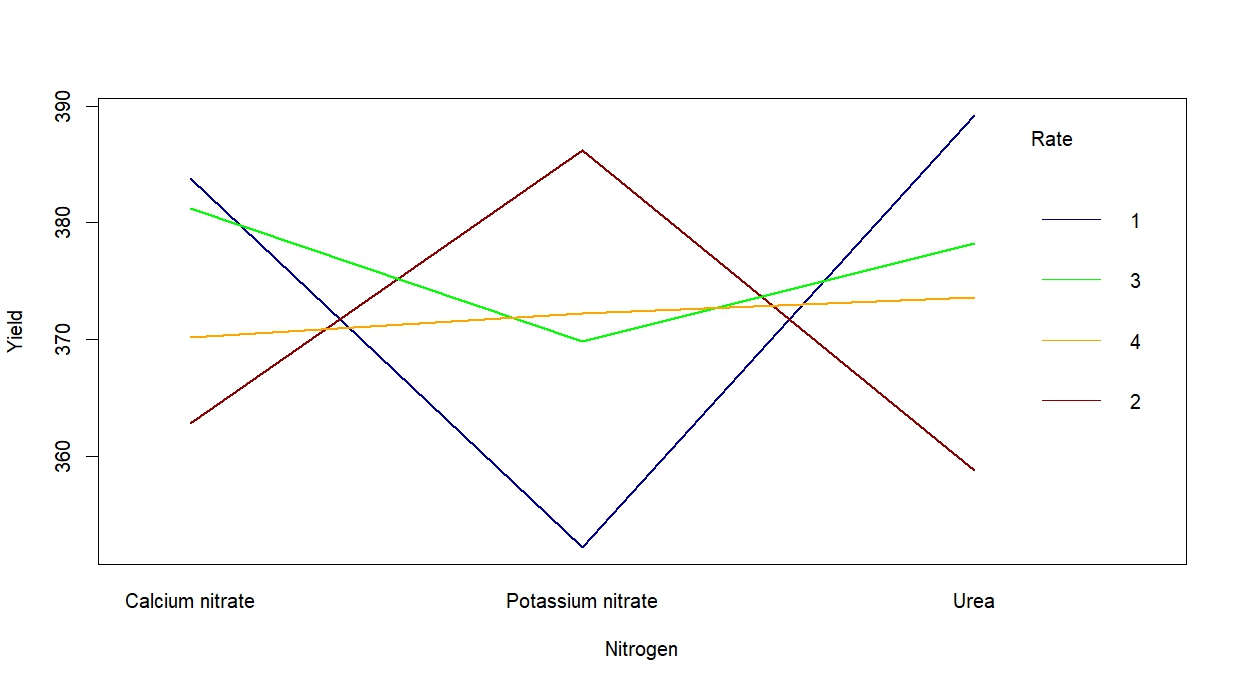
\includegraphics[width=0.7\linewidth]{prob5_inter}
	\caption[prob5_int]{Gráfico de interacción Rate*Nitrogen.}
	\label{fig:prob5inter}
\end{figure}
\textcolor{blue}{De acuerdo a la gráfica anterior se puede observar una interacción entre todos los niveles, siendo mas evidente para el 1.}
\item Realice el análisis no paramétrico utilizando rangos alineados con ARtool.
\begin{MyVerbatim}
# Parcelas divididas (no parametrico) con ArTool #
# Análisis de varianza #
anova_rangos<- art(Yield ~ Nitrogen*Rate+ (1|blk),data=datos3)
anova(anova_rangos)
# Prueba de Tukey #
media<-artlm(anova_rangos,"Nitrogen:Rate")
marginal<-emmeans(media, ~Nitrogen*Rate)
marginal
pares<-pairs(marginal,adjust = "tukey")
pares
plot(marginal)
\end{MyVerbatim}
Resultando:
\begin{MyVerbatim}
> anova(anova_rangos)
Analysis of Variance of Aligned Rank Transformed Data

Table Type: Analysis of Deviance Table (Type III Wald F 
tests with Kenward-Roger df) 
Model: Mixed Effects (lmer)
Response: art(Yield)

F Df Df.res  Pr(>F)  
1 Nitrogen      0.19354  2     44 0.82473  
2 Rate          0.24031  3     44 0.86775  
3 Nitrogen:Rate 1.22255  6     44 0.31313  
---
Signif. codes:   0 ‘***’ 0.001 ‘**’ 0.01 ‘*’ 0.05 ‘.’ 0.1 ‘ ’ 1 
\end{MyVerbatim}
\textcolor{blue}{El análisis de la varianza evidencia que no existe diferencia estadisticamente significativa entre los factores y sus interacciones, ya que los pvalue son mayores al alfa utilizado (\(\alpha=0.05\)).\\
Al haberse rechazado la hipótesis y no existir diferencia estadística significativa, no se tendría caso realizar una prueba de comparación de medias
sin embargo; con fines didácticos se realiza la siguiente prueba.}
\begin{MyVerbatim}
# Prueba de Tukey #
media<-artlm(anova_rangos,"Nitrogen:Rate")
marginal<-emmeans(media, ~Nitrogen*Rate)
marginal
pares<-pairs(marginal,adjust = "tukey")
pares
plot(marginal)+theme_pubr()
\end{MyVerbatim}
Resultando:
\begin{MyVerbatim}
> marginal
Nitrogen          Rate emmean  SE   df lower.CL upper.CL
Calcium nitrate   1      34.0 8.1 45.6    17.69     50.3
Potassium nitrate 1      18.2 8.1 45.6     1.89     34.5
Urea              1      38.2 8.1 45.6    21.89     54.5
Calcium nitrate   2      26.2 8.1 45.6     9.89     42.5
Potassium nitrate 2      42.4 8.1 45.6    26.09     58.7
Urea              2      23.4 8.1 45.6     7.09     39.7
Calcium nitrate   3      32.8 8.1 45.6    16.49     49.1
Potassium nitrate 3      29.7 8.1 45.6    13.39     46.0
Urea              3      30.6 8.1 45.6    14.29     46.9
Calcium nitrate   4      29.1 8.1 45.6    12.79     45.4
Potassium nitrate 4      32.8 8.1 45.6    16.49     49.1
Urea              4      28.6 8.1 45.6    12.29     44.9
	
Degrees-of-freedom method: kenward-roger 
Confidence level used: 0.95 
> pares
contrast                           estimate SE df t.ratio p.value
CalciumN Rate1 - PotassiN Rate1     15.8 11 44   1.430  0.9508
CalciumN Rate1 - Urea Rate1         -4.2 11 44  -0.380  1.0000
CalciumN Rate1 - CalciumN Rate2      7.8 11 44   0.706  0.9999
CalciumN Rate1 - PotassiNRate2      -8.4 11 44  -0.760  0.9997
CalciumN Rate1 - Urea Rate2         10.6 11 44   0.959  0.9979
CalciumN Rate1 - CalciumN Rate3      1.2 11 44   0.109  1.0000
CalciumN Rate1 - PotassiN Rate3      4.3 11 44   0.389  1.0000
CalciumN Rate1 - Urea Rate3          3.4 11 44   0.308  1.0000
CalciumN Rate1 - CalciumN Rate4      4.9 11 44   0.443  1.0000
CalciumN Rate1 - PotassiN Rate4      1.2 11 44   0.109  1.0000
CalciumN Rate1 - Urea Rate4          5.4 11 44   0.489  1.0000
PotassiN Rate1 - Urea Rate1         20.0 11 44  -1.810  0.8039
PotassiN Rate1 - CalciumN Rate2     -8.0 11 44  -0.724  0.9998
PotassiN Rate1 - PotassiN Rate2    -24.2 11 44  -2.190  0.5649
PotassiN Rate1 - Urea Rate2         -5.2 11 44  -0.471  1.0000
PotassiN Rate1 - CalciumN Rate3    -14.6 11 44  -1.321  0.9717
PotassiN Rate1- PotassiN Rate3     -11.5 11 44  -1.041  0.9957
PotassiN Rate1- Urea Rate3         -12.4 11 44  -1.122  0.9919
PotassiN Rate1- CalciumN Rate4     -10.9 11 44  -0.986  0.9973
PotassiN Rate1- PotassiN Rate4     -14.6 11 44  -1.321  0.9717
PotassiN Rate1- Urea Rate4         -10.4 11 44  -0.941  0.9982
Urea Rate1 - CalciumN Rate2         12.0 11 44   1.086  0.9938
Urea Rate1 - PotassiN Rate2         -4.2 11 44  -0.380  1.0000
Urea Rate1 - Urea Rate2             14.8 11 44   1.339  0.9687
Urea Rate1 - CalciumN Rate3          5.4 11 44   0.489  1.0000
Urea Rate1 - PotassiN Rate3          8.5 11 44   0.769  0.9997
Urea Rate1 - Urea Rate3              7.6 11 44   0.688  0.9999
Urea Rate1 - CalciumN Rate4          9.1 11 44   0.824  0.9995
Urea Rate1 - PotassiN Rate4          5.4 11 44   0.489  1.0000
Urea Rate1 - Urea Rate4              9.6 11 44   0.869  0.9991
CalciumN Rate2 - PotassiN Rate2    -16.2 11 44  -1.466  0.9420
CalciumN Rate2 - Urea Rate2          2.8 11 44   0.253  1.0000
CalciumN Rate2 - CalciumN Rate3     -6.6 11 44  -0.597  1.0000
CalciumN Rate2 - PotassiN Rate3      3.5 11 44  -0.317  1.0000
CalciumN Rate2 - Urea Rate3         -4.4 11 44  -0.398  1.0000
CalciumN Rate2 - CalciumN Rate4     -2.9 11 44  -0.262  1.0000
CalciumN Rate2 - PotassiN Rate4     -6.6 11 44  -0.597  1.0000
CalciumN Rate2 - Urea Rate4         -2.4 11 44  -0.217  1.0000
PotassiN Rate2 - Urea Rate2         19.0 11 44   1.720  0.8496
PotassiN Rate2 - CalciumN Rate3      9.6 11 44   0.869  0.9991
PotassiN Rate2 - PotassiN Rate3     12.7 11 44   1.149  0.9902
PotassiN Rate2 - Urea Rate3         11.8 11 44   1.068  0.9946
PotassiN Rate2 - CalciumN Rate4     13.3 11 44   1.204  0.9859
PotassiN Rate2 - PotassiN Rate4      9.6 11 44   0.869  0.9991
PotassiN Rate2 - Urea Rate4         13.8 11 44   1.249  0.9813
Urea Rate2 - CalciumN Rate3         -9.4 11 44  -0.851  0.9993
Urea Rate2 - PotassiN Rate3         -6.3 11 44  -0.570  1.0000
Urea Rate2 - Urea Rate3             -7.2 11 44  -0.652  0.9999
Urea Rate2 - CalciumN Rate4         -5.7 11 44  -0.516  1.0000
Urea Rate2 - PotassiN Rate4         -9.4 11 44  -0.851  0.9993
Urea Rate2 - Urea Rate4             -5.2 11 44  -0.471  1.0000
CalciumN Rate3 - PotassiN Rate3      3.1 11 44   0.281  1.0000
CalciumN Rate3 - Urea Rate3          2.2 11 44   0.199  1.0000
CalciumN Rate3 - CalciumN Rate4      3.7 11 44   0.335  1.0000
CalciumN Rate3 - PotassiN Rate4      0.0 11 44   0.000  1.0000
CalciumN Rate3 - Urea Rate4          4.2 11 44   0.380  1.0000
PotassiN Rate3 - Urea Rate3         -0.9 11 44  -0.081  1.0000
PotassiN Rate3 - CalciumN Rate4      0.6 11 44   0.054  1.0000
PotassiN Rate3 - PotassiN Rate4     -3.1 11 44  -0.281  1.0000
PotassiN Rate3 - Urea Rate4          1.1 11 44   0.100  1.0000
Urea Rate3 - CalciumN Rate4          1.5 11 44   0.136  1.0000
Urea Rate3 - PotassiN Rate4         -2.2 11 44  -0.199  1.0000
Urea Rate3 - Urea Rate4              2.0 11 44   0.181  1.0000
CalciumN Rate4 - PotassiN Rate4     -3.7 11 44  -0.335  1.0000
CalciumN Rate4 - Urea Rate4          0.5 11 44   0.045  1.0000
PotassiN Rate4 - Urea Rate4          4.2 11 44   0.380  1.0000

Degrees-of-freedom method: kenward-roger 
P value adjustment: tukey method for comparing a family of 12 estimates 
\end{MyVerbatim}
\textcolor{blue}{La prueba anterior muestra que no existe diferencia entre las entre las interacciones, ya que todos los p-value son 1 o cercanos a 1}
\begin{figure}[H]
	\centering
	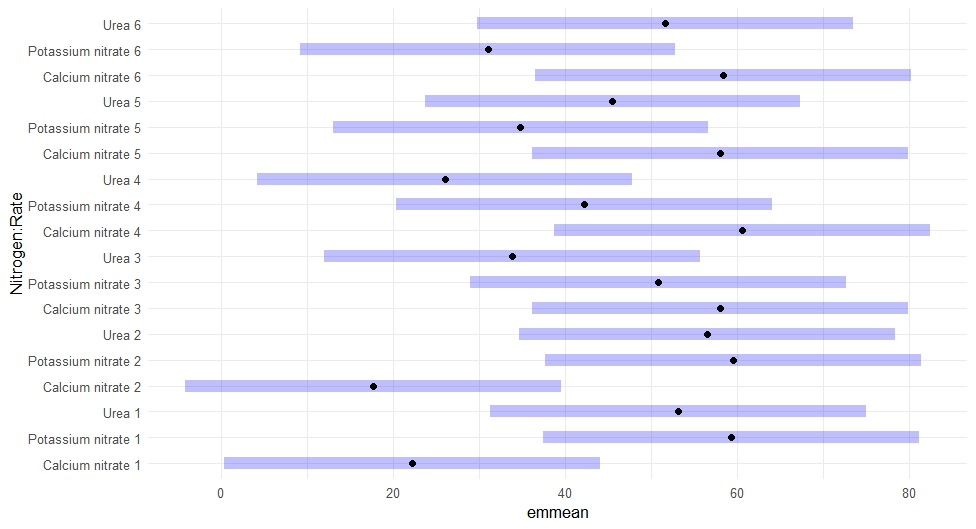
\includegraphics[width=0.7\linewidth]{prob5_mediu}
	\caption[prob5_mediu]{Comparación de medias}
	\label{fig:prob5mediu}
\end{figure}

\textcolor{blue}{En el gráfico anterior se muestra la comparación de medias entre los niveles del factor Nitrógeno, evidenciando que no existe una diferencia estadística significativa}

	\end{enumerate}
\newpage
%%%%%%%%%%%%%%%%%%%%%%%%%%%%%%%%%%%%%%%%%%%%%%%%%%%%%%%%%%%%%%
\section*{Problema 6}
Los machos de la magnífica fragata (\textit{Fregata magnificens}) tienen una gran bolsa roja en la garganta. Muestran visualmente esta bolsa y la usan para emitir un sonido de tambor cuando buscan pareja. Madsen et al. (2004) querían saber si las hembras, que presumiblemente eligen pareja en función del tamaño de su bolsa, podían utilizar el tono del sonido del tambor como indicador del tamaño de su bolsa. Los autores estimaron el volumen de la bolsa y la frecuencia fundamental del sonido del tambor en 18 machos.
\begin{center}
	\begin{table}[H]
		\centering
		\caption{Volumen de bolsa y Frecuencia fundamental emitida.}
		\begin{tabular}{cc}
			\toprule[1.5 pt]
			Volume ($cm^3$) & Frecuency (Hz) \\
			\midrule
			1760&529\\
			2040&566\\
			2440&473\\
			2550&461\\
			2730&465\\
			2740&532\\
			3010&484\\
			3080&527\\
			3370&488\\
			3740&485\\
			4910&478\\
			5090&434\\
			5090&468\\
			5380&449\\
			5850&425\\
			6730&389\\
			6990&421\\
			7960&416\\
			\bottomrule[1.5pt]
		\end{tabular}
		\label{tab:my_label6}
	\end{table}
\end{center}

\begin{enumerate} [label=\textbf{\alph*})]
\item \textbf{Realice una gráfica X vs Y.}
\begin{MyVerbatim}
dat<-read.csv("prob6.csv", header=T)
Frequencia<-dat\$freq
Volumen<-dat\$volume
attach(dat)
str(dat)
cor(Volumen,Frequencia)
plot(Volumen,Frequencia)
\end{MyVerbatim}
\begin{figure}[H]
	\centering
	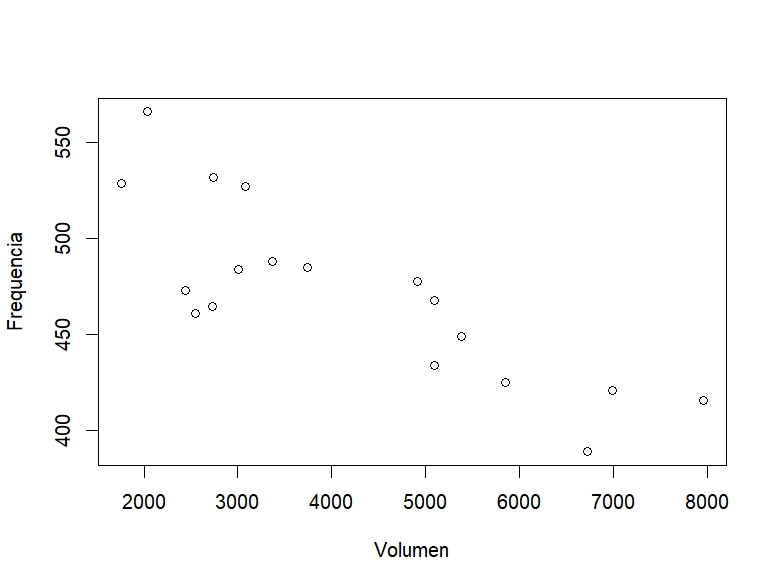
\includegraphics[width=0.7\linewidth]{corr_prob6}
	\caption[cor\_prob6]{Gráfica x \& y de la Frecuencia emitida y el Volumen.}
	\label{fig:corrprob6}
\end{figure}
\item \textbf{Obtenga el coeficiente de correlación de Spearman, Kendall y de Pearson. Interprete.}
\begin{MyVerbatim}
# Paramétrica #
cor(Volumen, Frecuencia)

# No paramétrica #
# Spearman Test #
	cor.test(Volumen,Frequencia, method = "spearman")
# Kendall Test #
	cor.test(Volumen, Frequencia, method ="kendall")
\end{MyVerbatim}
Resultando:
\begin{MyVerbatim}
Pearson's product-moment correlation

data:  Volumen and Frequencia
t = -5.7375, df = 16, p-value = 3.056e-05
alternative hypothesis: true correlation is not equal to 0
95 percent confidence interval:
-0.9307345 -0.5728357
sample estimates:
cor 
-0.8203196 

Spearman's rank correlation rho

data:  Volumen and Frequencia
S = 1708.4, p-value = 0.0002302
alternative hypothesis: true rho is not equal to 0
sample estimates:
rho 
-0.7630357 

Kendall's rank correlation tau

data:  Volumen and Frequencia
z = -3.5631, p-value = 0.0003666
alternative hypothesis: true tau is not equal to 0
sample estimates:
tau 
-0.6163968 
\end{MyVerbatim} 
\end{enumerate}
\textcolor{blue}{En todos los tests, se pudo evidenciar una correlación entre ambas variables (Volumen y Frecuencia), ya que los coeficientes son mayores a 0.5 y el p- value en todos los casos fue menor al alfa (\(\alpha=0.5\)). De igual manera, esta correlación en todos los casos siempre fue negativa. Por lo que se concluye que existe una correlación negativa entre ambas variables.}
\newpage
%%%%%%%%%%%%%%%%%%%%%%%%%%%%%%%%%%%%%%%%%%%%%%%
\section*{Problema 7}
Del trabajo:\\
\\KOKLU, M. and OZKAN, I.A., (2020), Multiclass Classification of Dry Beans Using Computer Vision and Machine Learning Techniques. \textit{Computers and Electronics in Agriculture}, 174, 105507.
https://doi.org/10.1016/j.compag.2020.105507.\\
\\En esta investigación se utilizaron siete diferentes variedades de frijoles secos, teniendo en cuenta las características como forma, aspecto, tipo y estructura según la situación del mercado. Se desarrolló un sistema de visión por computadora para distinguir siete variedades diferentes registradas de frijol seco con características similares para obtener una clasificación uniforme de semillas. Para el modelo de clasificación se tomaron imágenes de 13,611 granos de siete variedades de granos de frijol secos diferentes registrados con una cámara de alta resolución. Las imágenes de frijoles obtenidas por el sistema de visión por computadora 8 se sometieron a etapas de segmentación y extracción de características, y un total de 16 características; De los granos se obtuvieron 12 dimensiones y 4 formas.
\begin{enumerate} [label=\textbf{\alph*})]
\item Realice un análisis de correlación para investigar la relacion entre atributos de las semillas de frijol utilizando los coeficientes de Pearson, Spearman y Kendall, interprete sus resultados. Los atributos presentan normalidad.\\
\textcolor{blue}{\\Como primer paso para abordar el problema se necesita corroborar la normalidad de los datos y conocer su distribución. Dado que el numero de observaciones supera 10,000 (y para la prueba se sugiere se maneje en un rango de 3 a 5000 observaciones) se utilizó el paquete \textit{skim} para desglosar los atributos y de una manera visual poder identificar con un histograma dicha normalidad. Este es un método rudimentario en la exploración, sin embargo para apoyar estadisticamente los resultados se debe correr la prueba de Shapiro Wilk. }
	\begin{MyVerbatim}
# Datos #
dat7<-read.csv("prob7.csv",header = T)
View(dat7)
# Librerias #
library(ggplot2)
library(skimr)
# Explorar los datos #
glimpse(dat7)
dat7<- as.data.frame(lapply(dat7[,-17], as.numeric))
# Comprobar normalidad de los datos  #
skim(dat7[,-17])
	\end{MyVerbatim}
\begin{figure}[H]
	\centering
	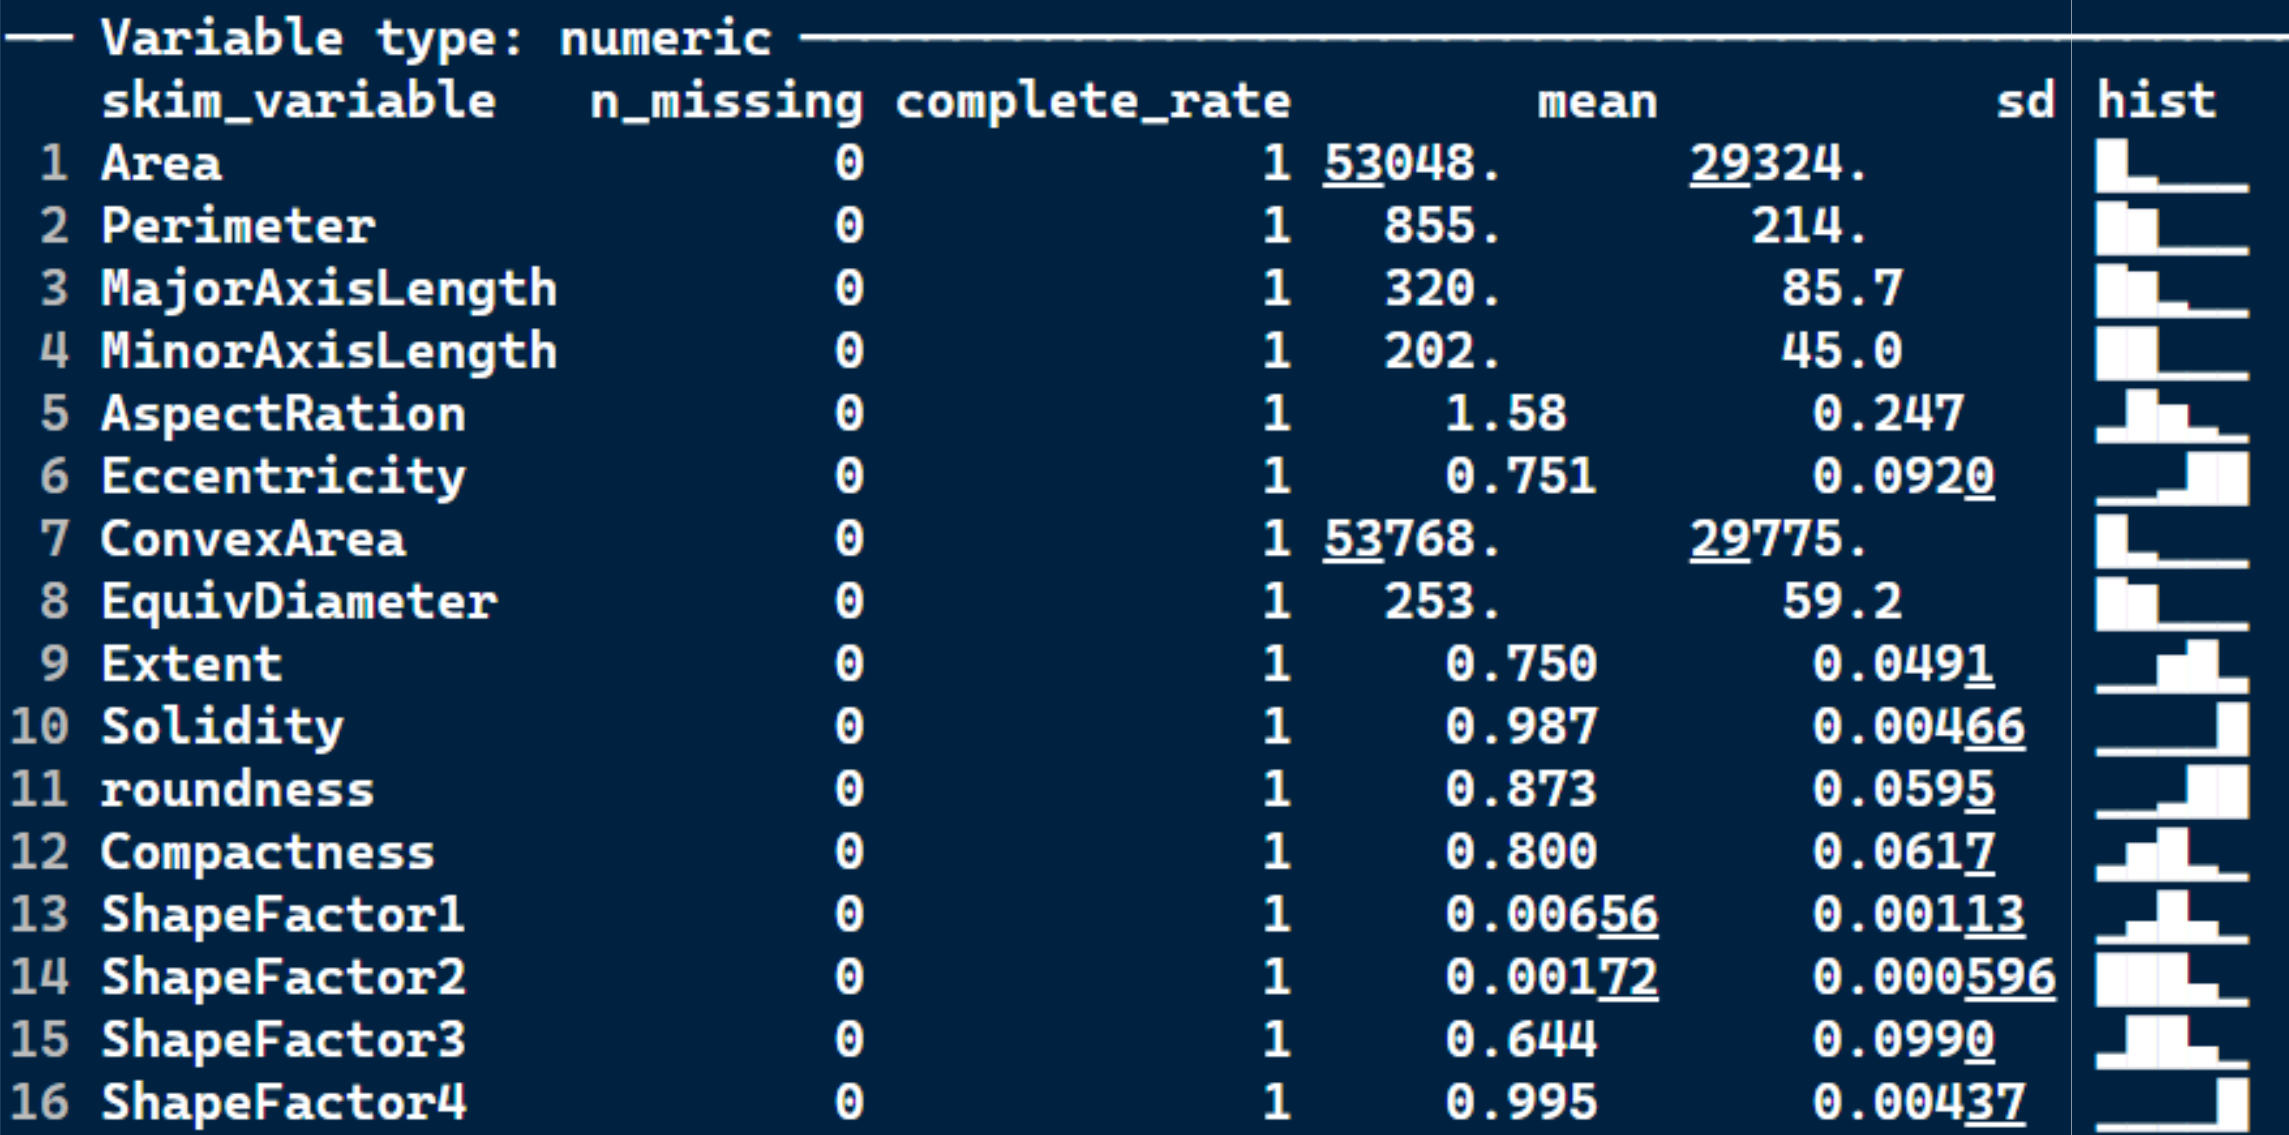
\includegraphics[width=0.7\linewidth]{prob7_hist}
	\caption[prob7-hist]{Exploración de los datos con \textit{skim} e histogramas de la distribución de los datos en cada variable.}
	\label{fig:prob7hist}
\end{figure}
\textcolor{blue}{De esta manera se puede suponer que los datos no cumplen con el supuesto de normalidad, pues la distribución de los datos en los histogramas no muestra ese comportamiento.\\
\\Para comprobar correlación de los datos y no habiendo rechazado la normalidad de los datos, se corrieron las pruebas de correlación parametricas (Pearson) y no paramétricas (Spearman, Kendall).}
\begin{MyVerbatim}
# Correlación de los datos #
library(corrplot)
# Nivel de confiabilidad #
testRes <- cor.mtest(copy_dat7, conf.level = 0.95)

# Parametrico (Pearson) #
P <- dat7 %>% 
select(where(is.numeric)) %>% 
cor()
round(P, 2)

corrplot(P, p.mat = testRes$p, method = 'circle', type = 'lower', 
insig='blank', tl.col = 'black', addCoef.col ='black',tl.cex= .8, 
number.cex = 0.6, order = 'AOE', diag=FALSE,
cl.ratio = 0.2, tl.srt = 45, col = COL2('PiYG', 10),number.font = 1.5)
title("Correlación de Pearson")
\end{MyVerbatim}
\begin{figure}[H]
	\centering
	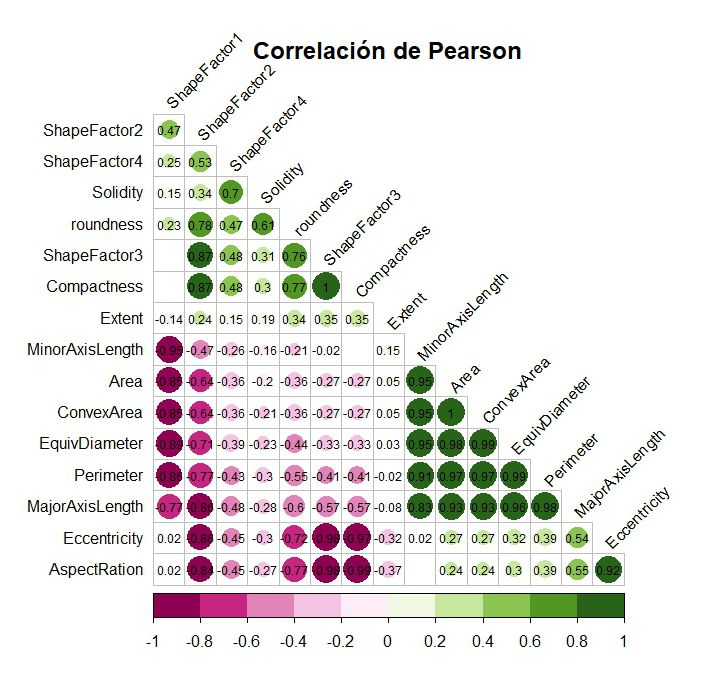
\includegraphics[width=0.7\linewidth]{prob7_corrPear}
	\caption[corr_pear]{Coeficientes de correlación de Pearson.}
	\label{fig:prob7corrpear}
\end{figure}

\begin{MyVerbatim}
# Spearmann #
R <- dat7 %>% 
select(where(is.numeric)) %>% 
cor(method = 'spearman')
round(R, 2)

corrplot(R, p.mat = testRes$p, method = 'circle', type = 'lower', 
insig='blank', tl.col = 'black', addCoef.col ='black',tl.cex= .8, 
number.cex = 0.6, order = 'AOE', diag=FALSE,
cl.ratio = 0.2, tl.srt = 45, col = COL2('PiYG', 10),number.font = 1.5)
title("Correlación de Spearmann")
\end{MyVerbatim}
\begin{figure}[H]
	\centering
	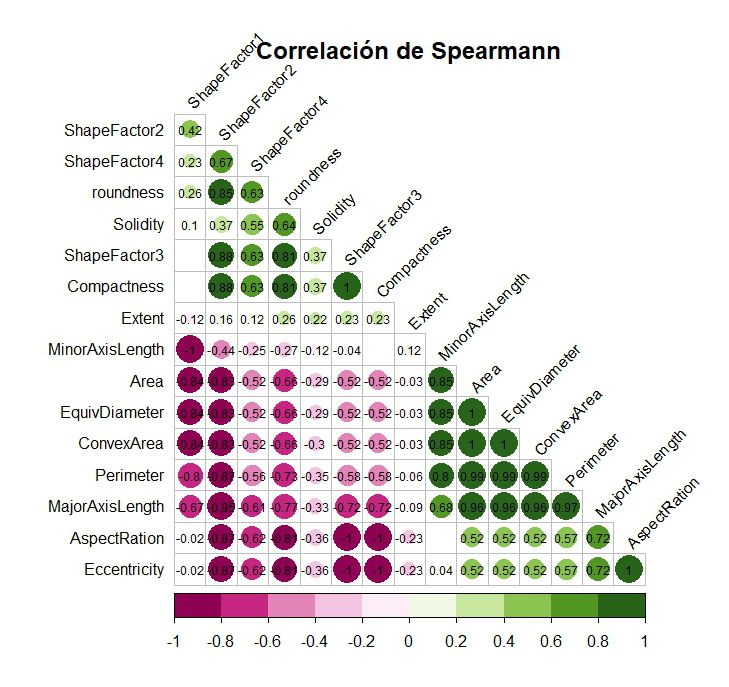
\includegraphics[width=0.7\linewidth]{prob7_corrSpear}
	\caption[corr_Spear]{Coeficientes de correlación de Spearman.}
	\label{fig:prob7corrspear}
\end{figure}
\begin{MyVerbatim}
# Kendall #
K <- dat7 %>% 
select(where(is.numeric)) %>% 
cor(method = 'kendall')
round(K, 2)

corrplot(K, p.mat = testRes$p, method = 'circle', type = 'lower', 
insig='blank', tl.col = 'black', 
addCoef.col ='black',tl.cex= .8, number.cex = 0.6, 
order = 'AOE', diag=FALSE, cl.ratio = 0.2, 
tl.srt = 45, col = COL2('PiYG', 10),number.font = 1.5)
title("Correlación de Kendall")
\end{MyVerbatim}
\begin{figure}[H]
	\centering
	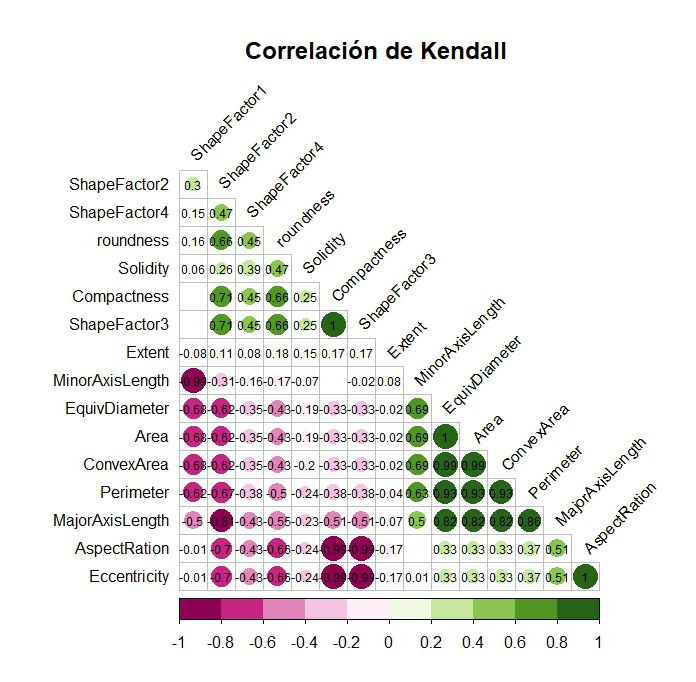
\includegraphics[width=0.7\linewidth]{prob7_corrKend}
	\caption[corr_kend]{Coeficientes de correlación de Kendall.}
	\label{fig.prob7corrkend}
\end{figure}

\textcolor{blue}{Para estos datos, las pruebas de correlación coinciden mostrando indices similares y comportamientos positivos negativos y positivos en las mismas variables, estas variables como: ConvexArea, EquivDiameter, Area, MajorAxisLength, AspectRation y Eccentricity.}
\item Investigue que atributos pueden detectar mejor la diferencia entre variedades de frijol, use Kruskall Wallis o tranformación a rangos de Conover \(\alpha=0.05\).\\
\\\textcolor{blue}{De acuerdo a los resultados anteriores las variables que mejor pueden detectar una diferencia entre las variedades de frijol son : ConvexArea, EquivDiameter, Area, MajorAxisLength, AspectRation, Eccentricity y Perimeter.}  
\\Para conocer si existe una diferencia entre las variedades, para las pruebas se utilizara la varible "Perimeter", dado que muestra una mayor cantidad de correlación con las demas variables. 
\begin{MyVerbatim}
# Test de Kruscakl-Wallis #
kruskal.test(Perimeter ~ Class, data = dat7)	
\end{MyVerbatim} 
Resultado:

\begin{MyVerbatim}
Kruskal-Wallis rank sum test

data:  Perimeter by Class
Kruskal-Wallis chi-squared = 11891, df = 6, p-value < 2.2e-16
\end{MyVerbatim}
\textcolor{blue}{Con un \(\alpha=0.5\), y un p-value de < 2.2e-16 se confirma existen diferencias estadísticamente significativas entre las distintas variedades.}
\item Realice las gráficas que apoyen su interpretación.\\
\\\textcolor{blue} {En la Figura 10, se puede evidenciar la diferencia entre las variedades, siendo la variedad \textit{Bombay} la que obtuvo un valor alto en comparación a las demás variedades.}
\begin{MyVerbatim}
ggboxplot(dat7, x = "Class", y = "Perimeter", 
color = "Class", palette = "jco", 
ylab = "Perimeter", xlab = "Class",)+
geom_jitter(color="black", size=0.4, alpha=0.9)+
theme_pubr()	
\end{MyVerbatim}
\begin{figure}[H]
	\centering
	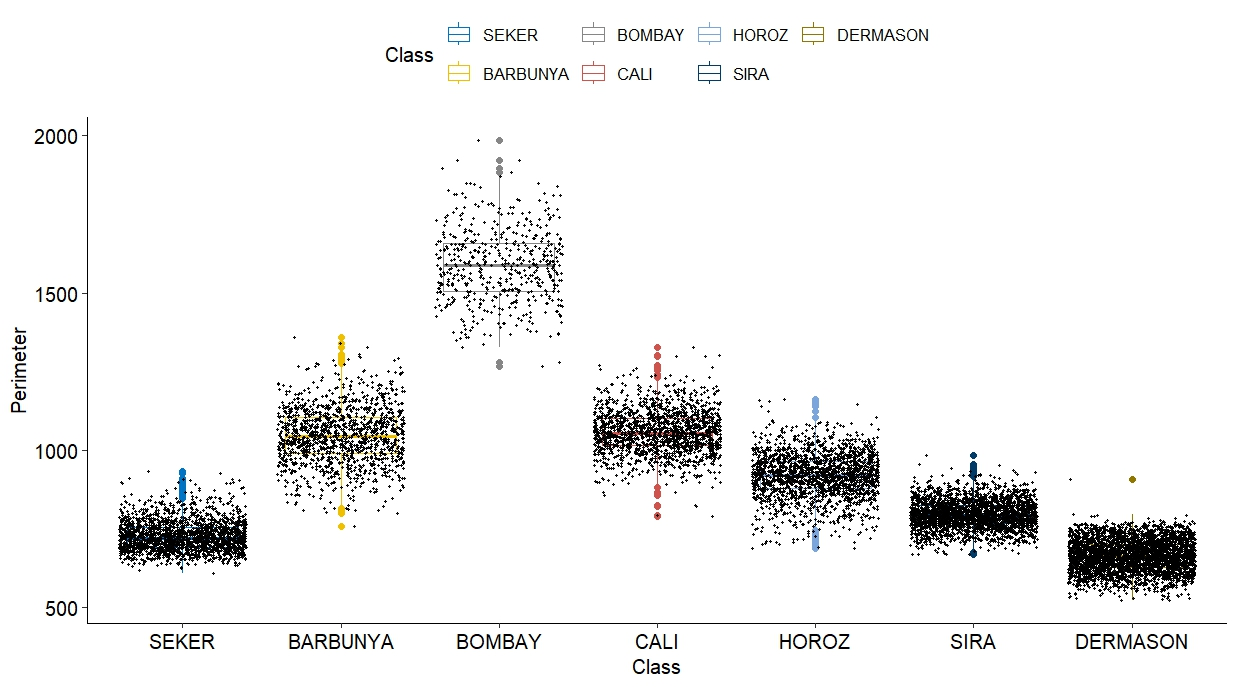
\includegraphics[width=0.7\linewidth]{prob7_boxfrij}
	\caption[prob7_boxfrij]{Variedades de Frijol respecto a la variable \textit{Perimeter}.}
	\label{fig.prob7boxfrij}
\end{figure}

\end{enumerate}
\end{document}
